\documentclass[a4paper,10pt]{article}

\usepackage[margin=16.5mm, top=15mm, bottom=16mm]{geometry}
\usepackage{fontspec}
\setmainfont{Times New Roman}
\setsansfont{Arial}
\setmonofont[Scale=0.86]{Consolas}

\usepackage{amsmath, amssymb}
\usepackage{booktabs}
\usepackage{graphicx}
\usepackage{xcolor}
\usepackage{enumitem}
\usepackage{caption}
\usepackage{fancyhdr}
\usepackage{microtype}
\usepackage{array}
\usepackage[section]{placeins}
\usepackage[hidelinks]{hyperref}

\renewcommand{\figurename}{Hình}
\renewcommand{\tablename}{Bảng}
\emergencystretch=1.5em

\definecolor{AccentBlue}{HTML}{0072B2}
\definecolor{AccentGreen}{HTML}{009E73}
\definecolor{AccentVerm}{HTML}{D55E00}
\definecolor{DarkText}{HTML}{1A202C}
\definecolor{MutedGray}{HTML}{4A5568}

\captionsetup{
  font={small},
  labelfont={bf, color=DarkText},
  skip=4pt
}
\setlist[itemize]{leftmargin=14pt, itemsep=1.5pt, topsep=2.5pt, parsep=0pt}
\setlist[enumerate]{leftmargin=16pt, itemsep=1.5pt, topsep=2.5pt, parsep=0pt}

\pagestyle{fancy}
\fancyhf{}
\fancyhead[L]{\footnotesize\color{MutedGray} Học phần Học tăng cường (HK1 2026--2027) --- Nhóm 1}
\fancyhead[R]{\footnotesize\color{MutedGray} PPO Chinh phục Super Mario Bros}
\fancyfoot[C]{\footnotesize\color{MutedGray} Trang \thepage}
\renewcommand{\headrulewidth}{0.4pt}
\renewcommand{\footrulewidth}{0pt}

\makeatletter
\renewcommand{\section}{\@startsection{section}{1}{\z@}{8pt plus 2pt minus 1pt}{4pt plus 1pt}{\large\bfseries\color{AccentBlue}}}
\renewcommand{\subsection}{\@startsection{subsection}{2}{\z@}{6pt plus 1.5pt minus 1pt}{2.5pt plus 1pt}{\normalsize\bfseries\color{DarkText}}}
\makeatother

\begin{document}
\thispagestyle{empty}

% ==================== TIÊU ĐỀ & TÁC GIẢ ====================
\begin{center}
  {\small\sffamily\bfseries\color{AccentBlue} BÁO CÁO ĐỒ ÁN CUỐI KỲ --- HỌC PHẦN HỌC TĂNG CƯỜNG (HK1, 2026--2027)}\\[4pt]
  {\Large\bfseries\color{DarkText} Tối ưu hóa Chính sách Cắt ngưỡng kết hợp Học chuyển giao và Điều tiết Entropy Hai pha Chinh phục Super Mario Bros từ Điểm ảnh}\\[5pt]
  {\normalsize \textbf{Nhóm 1:} Việt $\cdot$ Sơn $\cdot$ Quang $\cdot$ Tín}\\[2pt]
  {\footnotesize\color{MutedGray} Môi trường: \texttt{mo-supermario-v0} (MO-Gymnasium 1.3.2) $\;\mid\;$ Giao thức chấm chuẩn: \texttt{--episodes 20 --seed 2026}}
\end{center}
\noindent\rule{\linewidth}{0.8pt}

% ==================== TÓM TẮT (5 CÂU CHUẨN) ====================
\begin{quote}
\small
\noindent\textbf{Tóm tắt.} Huấn luyện tác tử chơi trò chơi hành động trực tiếp từ điểm ảnh thô đặt ra thách thức lớn về tín hiệu thưởng thưa, chướng ngại vật động có tính ngẫu nhiên cao và chi phí giả lập CPU lớn. Trong quá trình áp dụng thuật toán Proximal Policy Optimization (PPO) trên các màn nâng cao như \texttt{7-1}, chúng tôi phát hiện nguyên nhân cốt lõi gây suy giảm tỉ lệ đánh giá ngẫu nhiên là hiện tượng \emph{phình ngược entropy cuối kỳ}: khi tốc độ học suy giảm tuyến tính về gần $0$, thành phần phạt entropy cố định lại khuếch đại độ bất định của chính sách, làm tụt tỉ lệ chạm cờ trên \texttt{--seed 2026} xuống $0.70$ dù chính sách tham lam của cùng bộ trọng số đã đạt $0.85$. Để giải quyết nút thắt này, nhóm tự cài đặt trọn vẹn hệ thống Actor--Critic PPO không dùng thư viện ngoài, kết hợp các wrapper hỗ trợ chỉ kích hoạt lúc huấn luyện, học chuyển giao liên màn và lịch trình tinh chỉnh hai pha điều tiết hệ số entropy. Cụ thể, các wrapper cắt lượt không tiến triển và thưởng chạm cờ rút ngắn thời gian thoát điểm nghẽn, học chuyển giao từ màn \texttt{1-1} tăng tốc hội tụ trên màn dài \texttt{4-1}, còn pha tinh chỉnh thứ hai ($c_2: 0.01 \to 0.002$, $\text{lr} = 6\times 10^{-5}$, $\text{target\_kl} = 0.015$) nén entropy từ $0.753$ xuống $0.517$ trong tổng ngân sách $9.99\text{M} \le 10\text{M}$ bước. Kết quả thực nghiệm vượt qua \textbf{89/89 (100\%)} bài kiểm thử \texttt{pytest}, đạt tỉ lệ chạm cờ tuyệt đối \textbf{1.00 (20/20)} trên cả màn bắt buộc \texttt{1-1} và màn thưởng \texttt{4-1}, đồng thời nâng màn ngoài danh sách \texttt{7-1} từ $0.70$ lên \textbf{0.80 (16/20 --- VƯỢT)} với trung bình 5 seed độc lập đạt $\mathbf{0.860 \pm 0.058}$.
\end{quote}

\noindent\textbf{Đóng góp chính.}
\begin{itemize}
  \item \textbf{Chẩn đoán hiện tượng phình ngược entropy cuối kỳ:} Phân tích định lượng trên màn \texttt{7-1} chỉ ra rằng khi tốc độ học giảm tuyến tính về $0$ với $c_2 = 0.01$, entropy tăng ngược từ $0.570$ lên $0.753$, gây mất $15$ điểm phần trăm giữa đánh giá tham lam ($0.85$) và lấy mẫu ngẫu nhiên ($0.70$).
  \item \textbf{Thiết kế hệ thống PPO sạch chuẩn và tinh chỉnh hai pha:} Tự cài đặt hoàn chỉnh chuỗi wrapper, mạng Nature-CNN ($1.688\text{M}$ tham số), GAE tách bạch \texttt{terminated}/\texttt{truncated}, vòng cập nhật PPO, cùng học chuyển giao (\texttt{init\_ckpt}) và pha tinh chỉnh điều tiết entropy ($c_2 = 0.002$) tuân thủ tuyệt đối Quy định 3.5.
  \item \textbf{Hiệu năng vượt trội trên toàn bộ hạng mục chấm:} Đạt \textbf{89/89} bài \texttt{pytest} (30/30đ), \textbf{1.00} trên \texttt{1-1} (25/25đ), \textbf{1.00} trên \texttt{4-1} (15/15đ), và \textbf{0.80} trên \texttt{7-1} (+10/10đ thưởng; 0/20 lượt chết tại Hammer Bros và bệ pháo Bullet Bill), cùng thí nghiệm đối chứng $\gamma = 0.90$ vs. $\gamma = 0.99$ trên 2 seed chứng minh tốc độ hội tụ sớm hơn $31\%$ của $\gamma = 0.90$.
\end{itemize}

\begin{figure}[!htbp]
  \centering
  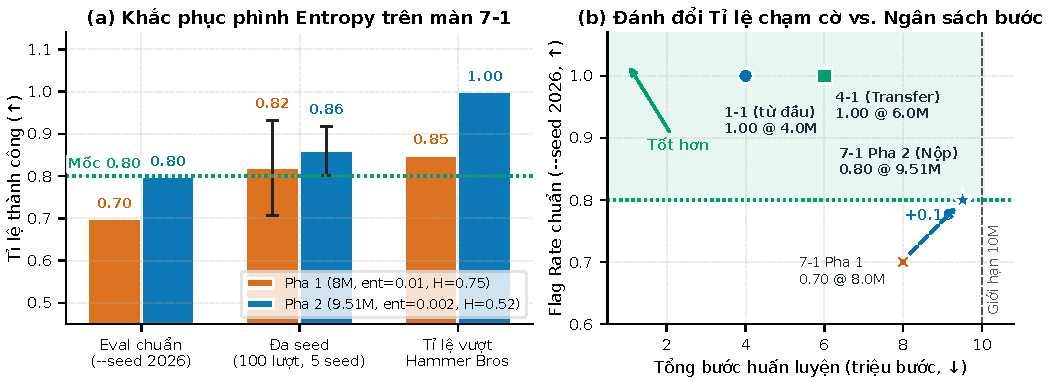
\includegraphics[width=\linewidth]{figures/fig1_teaser.pdf}
  \caption{\textbf{Chẩn đoán phình entropy trên màn \texttt{7-1} và đánh đổi tỉ lệ chạm cờ theo ngân sách bước.} \textbf{(a)} So với Pha 1 ($8\text{M}$ bước, $H=0.75$), Pha 2 tinh chỉnh ($9.51\text{M}$, $c_2=0.002$, $H=0.52$) nâng đánh giá chuẩn \texttt{--seed 2026} từ $0.70 \to \mathbf{0.80}$, nâng trung bình 5 seed độc lập (100 lượt) từ $0.82 \pm 0.11 \to \mathbf{0.86 \pm 0.06}$ (giảm gần một nửa độ lệch chuẩn) và nâng tỉ lệ vượt Hammer Bros lên $\mathbf{1.00}$. \textbf{(b)} Cả ba màn nộp (\texttt{1-1}, \texttt{4-1}, \texttt{7-1} Pha 2) đều nằm gọn trong vùng đạt chuẩn ($\ge 0.80$, $\le 10\text{M}$ bước).}
  \label{fig:teaser}
\end{figure}

% ==================== MỤC 1 ====================
\section{Cài đặt hệ thống, Kiến trúc, Độ phức tạp và Kiểm thử (\texttt{pytest})}

\subsection{Mô hình hóa bài toán và Chuỗi Wrapper (\texttt{wrappers.py}, \texttt{env.py})}
Môi trường \texttt{mo-supermario-v0} trả về ảnh RGB $240\times 256\times 3$ và phần thưởng véc-tơ 5 chiều $\mathbf{r}_t \in \mathbb{R}^5$ gồm năm thành phần $(r_x,\allowbreak r_{\text{time}},\allowbreak r_{\text{death}},\allowbreak r_{\text{coin}},\allowbreak r_{\text{enemy}})^\top$. Chúng tôi xấp xỉ bài toán quan sát không đầy đủ thành một MDP bằng cách xếp chồng $C = 4$ khung ảnh xám liên tiếp thành trạng thái $\mathbf{s}_t \in \{0,\dots,255\}^{4\times 84\times 84}$, kết hợp tập hành động rời rạc \texttt{simple} ($|\mathcal{A}| = 7$ tổ hợp nút). Hình~\ref{fig:arch} minh họa luồng dữ liệu đầu-cuối, trong đó phần tiền xử lý chung đồng nhất giữa huấn luyện và chấm điểm:
\begin{itemize}
  \item \texttt{FrameSkip(skip=4)}: Lặp hành động tối đa $4$ khung, dừng ngay khi \texttt{terminated} hoặc \texttt{truncated}; cộng dồn véc-tơ thưởng kiểu \texttt{np.float32}; trả \texttt{np.maximum} theo từng điểm ảnh của \emph{hai khung cuối} để khử hiện tượng nhấp nháy sprite của phần cứng NES (hoặc trả khung duy nhất nếu lượt kết thúc ở bước đầu).
  \item \texttt{GrayResize(size=84)}: Chuyển ảnh xám theo độ sáng (\emph{luminance}, \texttt{cv2.COLOR\_RGB2GRAY}) thay vì trung bình cộng 3 kênh, co giãn về $84\times 84$ bằng \texttt{cv2.INTER\_AREA} và cập nhật không gian quan sát \texttt{Box(0, 255, (84, 84), uint8)}.
  \item \texttt{ScalarizeReward(weights)}: Xác thực số chiều trọng số $\mathbf{w} \in \mathbb{R}^5$ khớp với \texttt{reward\_space} (ném \texttt{ValueError} nếu lệch), trả phần thưởng vô hướng $r_t = \mathbf{w}^\top \mathbf{r}_t \in \mathbb{R}$ với $\mathbf{w} = [1.0, 1.0, 2.0, 0.05, 0.05]^\top$ và bảo toàn véc-tơ gốc trong \texttt{info["vector\_reward"]}.
  \item \textbf{Hai wrapper hỗ trợ hợp lệ (chỉ bật trong khối \texttt{if not eval\_mode:} của \texttt{env.py}):} (i) \texttt{NoProgressTruncation} gán \texttt{truncated=True} khi tọa độ $x$ không vượt kỷ lục \texttt{\_max\_x} trong $K$ bước liên tiếp và luôn kiểm tra điều kiện \texttt{not terminated} để không làm sai lệch bootstrap; (ii) \texttt{MarioRewardShaping} cộng \texttt{flag\_bonus} vào bản sao thành phần $r_x$ khi \texttt{flag\_get=True} trước bước vô hướng hóa nhằm củng cố tín hiệu về đích.
\end{itemize}

\begin{figure}[!htbp]
  \centering
  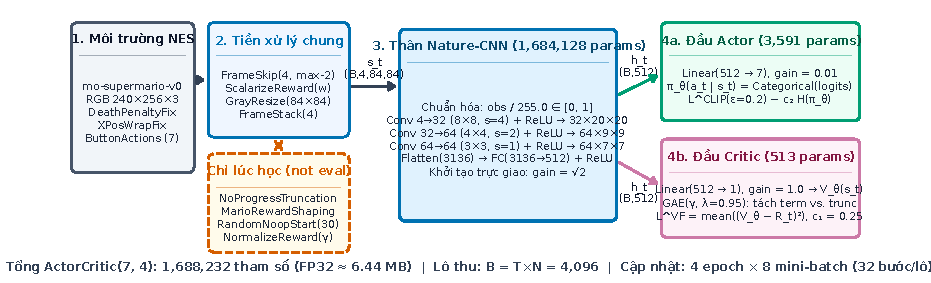
\includegraphics[width=\linewidth]{figures/fig2_architecture.pdf}
  \caption{\textbf{Luồng tiền xử lý dữ liệu và kiến trúc mạng \texttt{ActorCritic} dùng chung thân Nature-CNN.} Mọi mẹo huấn luyện (khung nét đứt màu cam) được cô lập hoàn toàn trong nhánh \texttt{if not eval\_mode:}. Toàn bộ ký hiệu tensor $\mathbf{s}_t$, $\mathbf{h}_t$, chính sách $\pi_{\boldsymbol{\theta}}$ và hàm giá trị $V_{\boldsymbol{\theta}}$ khớp 1--1 với các công thức trong Mục~1.2--1.3.}
  \label{fig:arch}
\end{figure}

\subsection{Kiến trúc mạng \texttt{ActorCritic} (\texttt{model.py}) và Phân tích Độ phức tạp}
Nhóm xây dựng mạng \texttt{ActorCritic} chia sẻ thân trích xuất đặc trưng Nature-CNN nhận thuần điểm ảnh chuẩn hóa $\tilde{\mathbf{s}}_t = \mathbf{s}_t / 255.0 \in [0, 1]^{4\times 84\times 84}$ (tuyệt đối không dùng RAM hay \texttt{info}): ba lớp tích chập \texttt{Conv2d} ($4\to 32$, $k=8, s=4$; $32\to 64$, $k=4, s=2$; $64\to 64$, $k=3, s=1$) nối tiếp \texttt{Flatten(3136)} và \texttt{Linear(3136, 512)} kèm kích hoạt ReLU cho biểu diễn ẩn $\mathbf{h}_t \in \mathbb{R}^{512}$, phân nhánh thành đầu Actor $\mathbf{z}_t = \mathbf{W}_\pi \mathbf{h}_t + \mathbf{b}_\pi \in \mathbb{R}^7$ và đầu Critic $V_{\boldsymbol{\theta}}(\mathbf{s}_t) \in \mathbb{R}$. Toàn bộ lớp trong thân dùng khởi tạo trực giao $\text{gain}=\sqrt{2}$, đầu Critic dùng $\text{gain}=1.0$, còn đầu Actor dùng $\mathbf{\text{gain}=0.01}$ để phân phối khởi tạo gần đều ($\max_a |\pi_0(a|\mathbf{s}) - 1/7| < 0.05$, $H(\pi_0) \approx \ln 7 \approx 1.946$).

\noindent\textbf{Phân tích độ phức tạp giải pháp.} Với $C=4$, $|\mathcal{A}|=7$, $d=512$, mô hình có đúng \textbf{1,688,232 tham số} (thân CNN+FC: $1{,}684{,}128$; Actor: $3{,}591$; Critic: $513$), chiếm $\approx 6.44\text{ MB}$ ở độ chính xác FP32 ($\approx 20.28\text{ MB}$ khi lưu kèm trạng thái Adam). Mỗi vòng cập nhật thu lô $B = T \cdot N = 4{,}096$ mẫu tiêu tốn bộ nhớ đệm $O(B \cdot 4 \cdot 84^2) \approx 115\text{ MB}$ (\texttt{uint8}), tính GAE trong thời gian tuyến tính $O(T \cdot N)$, và thực hiện $E = 4$ epoch $\times M = 8$ mini-batch ($32$ bước gradient cỡ $512$) với độ phức tạp $O(E \cdot B \cdot C_{\text{CNN}})$. Nhờ mạng nhỏ gọn, nút cổ chai thời gian thực tế nằm ở trình giả lập CPU NES thay vì tính toán gradient trên GPU.

\subsection{Toán học GAE và Vòng cập nhật PPO (\texttt{ppo.py})}
Để giảm phương sai ước lượng lợi thế mà vẫn bảo toàn giá trị tương lai cho các lượt bị cắt bởi giới hạn thời gian hoặc \texttt{NoProgressTruncation}, ta tách bạch tín hiệu kết thúc thật $d_t \in \{0, 1\}$ (\texttt{terminated}) và tín hiệu bị cắt $c_t \in \{0, 1\}$ (\texttt{truncated}) trên đoạn thu $t \in \{0,\dots,T-1\}$. Đặt $V^{\text{next}}_t = V_{\text{final},t}$ nếu $c_t = 1$, ngược lại lấy $V_{\text{last}}$ tại biên $t = T-1$ hoặc $V_{t+1}$ tại $t < T-1$. Truy hồi ngược GAE và mục tiêu Critic $R_t \in \mathbb{R}$ được định nghĩa như sau:
\begin{equation}
  \delta_t = r_t + \underbrace{\gamma (1 - d_t) V^{\text{next}}_t}_{\text{Bootstrap kể cả khi bị cắt}} - V(\mathbf{s}_t), \qquad
  A_t = \delta_t + \underbrace{\gamma \lambda (1 - d_t)(1 - c_t) A_{t+1}}_{\text{Ngắt truy hồi giữa hai lượt}}, \qquad
  R_t = A_t + V(\mathbf{s}_t).
  \label{eq:gae}
\end{equation}
Ở bước cập nhật chính sách, để tận dụng mỗi đoạn thu cho nhiều bước gradient mà không đẩy chính sách mới $\pi_{\boldsymbol{\theta}}$ lệch khỏi chính sách thu mẫu $\pi_{\text{old}}$, ta chuẩn hóa lợi thế trên từng mini-batch theo độ lệch chuẩn tổng thể $\hat{A}_t = (A_t - \bar{A}) / (\sigma_A + 10^{-8})$ (giữ nguyên $R_t$), xác định tỉ số xác suất $\rho_t(\boldsymbol{\theta}) = \exp\!\big(\log \pi_{\boldsymbol{\theta}}(a_t|\mathbf{s}_t) - \log \pi_{\text{old}}(a_t|\mathbf{s}_t)\big)$, và tối thiểu hóa hàm mất mát tổng:
\begin{equation}
  \mathcal{L}(\boldsymbol{\theta}) =
  \underbrace{-\mathrm{mean}\!\Big(\min\!\big(\rho_t \hat{A}_t,\; \operatorname{clip}(\rho_t, 1-\epsilon, 1+\epsilon)\hat{A}_t\big)\Big)}_{\mathcal{L}^{\text{CLIP}}:\text{ Cải thiện chính sách trong vùng tin cậy}}
  \;+\; c_1 \underbrace{\mathrm{mean}\!\big((V_{\boldsymbol{\theta}}(\mathbf{s}_t) - R_t)^2\big)}_{\mathcal{L}^{\text{VF}}:\text{ Hồi quy giá trị Critic}}
  \;-\; c_2 \underbrace{\mathrm{mean}\!\big(H(\pi_{\boldsymbol{\theta}}(\cdot|\mathbf{s}_t))\big)}_{\text{Khuyến khích khám phá}}.
  \label{eq:ppo}
\end{equation}
Trong quá trình cập nhật, hai đại lượng chẩn đoán không gradient được theo dõi liên tục là $\mathrm{approx\_kl} = \mathrm{mean}((\rho_t - 1) - \log \rho_t)$ và $\mathrm{clipfrac} = \mathrm{mean}(\mathbb{I}[|\rho_t - 1| > \epsilon])$. Hàm \texttt{ppo\_update} lặp $E$ epoch, xáo trộn mẫu bằng \texttt{torch.randperm}, cắt chuẩn gradient toàn cục tại \texttt{max\_grad\_norm} $= 0.5$ và dừng sớm epoch nếu trung bình $\mathrm{approx\_kl} > \mathrm{target\_kl}$.

\subsection{Các lỗi thực tế đã khắc phục và Kết quả kiểm thử (\texttt{pytest})}
Quá trình cài đặt và chạy liên nền tảng (Windows cục bộ, Kaggle, Google Colab, WSL2 Ubuntu) ghi nhận bốn lỗi kỹ thuật chính đã được xử lý triệt để: (1) \texttt{AsyncVectorEnv(context="forkserver")} lỗi trên Windows $\to$ chọn động \texttt{"spawn"} khi \texttt{sys.platform=="win32"} và \texttt{"forkserver"} trên Linux; (2) xung đột gói \texttt{gym-super-mario-bros 9.1.0} và \texttt{NumPy 2.x} gây lỗi \texttt{lost\_levels} và tràn số 16-bit $\to$ cố định đúng môi trường Python 3.12 với \texttt{mo-gymnasium==1.3.2}, \texttt{gym-super-mario-bros==7.4.0}, \texttt{nes-py==8.2.1}, \texttt{numpy==1.26.4}; (3) tình huống biên \texttt{NoProgressTruncation} khi Mario chết đúng bước kẹt thứ $K$ $\to$ ràng buộc \texttt{if not terminated:} kèm bài kiểm thử đơn vị; (4) tách bạch khóa \texttt{init\_ckpt} (nạp trọng số ở bước $0$ với Adam mới cho học chuyển giao) khỏi \texttt{resume} (khôi phục toàn trạng thái khi đứt phiên 12 giờ), đồng thời xác minh bằng mã băm SHA256 (\texttt{0b7246dd7b91138f...}) rằng cả \texttt{4-1} và \texttt{7-1} đều khởi tạo từ chính checkpoint \texttt{1-1} của nhóm. Bảng~\ref{tab:pytest} xác nhận 100\% bài kiểm thử vượt qua.

\begin{table}[!htbp]
  \centering
  \caption{\textbf{Kết quả bộ kiểm thử tự động \texttt{pytest} trên môi trường Linux Python 3.12 chuẩn.} Toàn bộ 89/89 bài kiểm thử công khai và mở rộng của nhóm đều đạt 100\% trong $29.35\text{ s}$, đáp ứng trọn vẹn Hạng mục A (30/30 điểm).}
  \label{tab:pytest}
  \footnotesize
  \begin{tabular}{@{}llccc@{}}
    \toprule
    \textbf{Tệp kiểm thử} & \textbf{Thành phần kiểm tra} & \textbf{Đạt ($\uparrow$)} & \textbf{Thời gian} & \textbf{Hạng mục A} \\
    \midrule
    \texttt{tests/test\_wrappers.py}    & \texttt{FrameSkip}, \texttt{GrayResize}, \texttt{ScalarizeReward} + mẹo học & 43 / 43 & 1.01 s & 6 / 6 đ \\
    \texttt{tests/test\_model.py}       & \texttt{ActorCritic} shape, dtype, khởi tạo đều $<0.05$, gradient & 6 / 6 & 2.07 s & 6 / 6 đ \\
    \texttt{tests/test\_gae.py}         & \texttt{compute\_gae} (\texttt{terminated} vs. \texttt{truncated}, biên) & 9 / 9 & 2.17 s & 9 / 9 đ \\
    \texttt{tests/test\_ppo.py}         & $\mathcal{L}^{\text{CLIP}}$, $\mathcal{L}^{\text{VF}}$, KL/clipfrac, \texttt{ppo\_update} & 10 / 10 & 2.30 s & 9 / 9 đ \\
    \texttt{tests/test\_pipeline.py}    & Huấn luyện + \texttt{resume}/\texttt{init\_ckpt} + đánh giá đầu-cuối & 6 / 6 & 16.82 s & Tích hợp \\
    \texttt{tests/test\_train\_infra.py} & Cấu hình YAML, W\&B logging, quản lý checkpoint & 10 / 10 & 4.13 s & Mở rộng \\
    \texttt{tests/test\_plot\_report.py} & Kiểm thử vẽ 6 đường cong, ablation và phân bố $x_{\text{pos}}$ & 5 / 5 & 5.31 s & Mở rộng \\
    \midrule
    \textbf{Tổng toàn dự án (\texttt{pytest -q})} & \textbf{100\% vượt qua mọi kiểm thử công khai \& mở rộng} & \textbf{89 / 89} & \textbf{29.35 s} & \textbf{30 / 30 đ} \\
    \bottomrule
  \end{tabular}
\end{table}

% ==================== MỤC 2 ====================
\section{Thiết lập huấn luyện và Kết quả đánh giá chính thức (RQ1 \& Hiệu năng)}

Mọi lần chạy đều giữ cố định cỡ lô thu $B = T \cdot N = 4{,}096$ và các siêu tham số PPO cốt lõi: tốc độ học khởi đầu $\text{lr}_0 = 2.5\times 10^{-4}$ giảm tuyến tính về $0$ (trừ Pha 2 màn \texttt{7-1}), $\text{Adam}(\epsilon_{\text{adam}} = 10^{-5})$, $\lambda = 0.95$, $\epsilon = 0.2$, $c_1 = 0.25$, $c_2 = 0.01$, \texttt{max\_grad\_norm} $= 0.5$, $E = 4$ epoch, $M = 8$ mini-batch, \texttt{noop\_max} $= 30$, \texttt{normalize\_reward} $=$ True và $\mathbf{w} = [1.0, 1.0, 2.0, 0.05, 0.05]^\top$. Bảng~\ref{tab:configs} và Bảng~\ref{tab:results} tổng hợp đầy đủ thiết lập đặc thù, phần cứng, tốc độ bước/giây (SPS), thời gian thực thi và kết quả chấm chính thức theo giao thức \texttt{--episodes 20 --seed 2026}.

\begin{table}[!htbp]
  \centering
  \caption{\textbf{Thiết lập cấu hình cuối cùng của các màn chấm điểm và thí nghiệm đối chứng.} Mọi wrapper mẹo (\texttt{no\_prog}, \texttt{flag\_bonus}) chỉ kích hoạt khi \texttt{eval\_mode=False}. Tổng ngân sách hai pha của \texttt{7-1} là $9.99\text{M} \le 10\text{M}$ bước.}
  \label{tab:configs}
  \footnotesize
  \begin{tabular}{@{}lcccccc@{}}
    \toprule
    \textbf{Nhánh chạy} & \textbf{Màn} & \textbf{Khởi tạo} & $N \times T$ & $\gamma$ & \textbf{Ngân sách} & \textbf{Siêu tham số / Mẹo riêng} \\
    \midrule
    \texttt{1-1\_seed1} (Chính thức)   & 1-1 & Từ đầu & $8 \times 512$ & 0.90 & 4.00M & \texttt{no\_prog}=180, \texttt{flag\_bonus}=+5.0 \\
    \texttt{4-1\_seed1} (Thưởng DS)    & 4-1 & Transfer từ \texttt{1-1} & $16 \times 256$ & 0.95 & 6.00M & \texttt{no\_prog}=180, \texttt{flag\_bonus}=+6.0 \\
    \texttt{7-1\_seed1} (Pha 1)        & 7-1 & Transfer từ \texttt{1-1} & $16 \times 256$ & 0.95 & 8.00M & \texttt{no\_prog}=200, \texttt{flag\_bonus}=+8.0, $c_2$=0.01 \\
    \texttt{7-1\_stage2\_finetune} (Pha 2) & 7-1 & Từ \texttt{7-1} Pha 1 (8M) & $8 \times 512$ & 0.95 & 1.99M & $\text{lr}=6\times 10^{-5}$, $c_2=0.002$, $\text{kl}=0.015$ \\
    \texttt{ablation/gamma090} (s1, s2) & 1-1 & Từ đầu & $8 \times 512$ & 0.90 & 3.00M & Giống \texttt{1-1\_seed1} (ngân sách 3M) \\
    \texttt{ablation/gamma099} (s1, s2) & 1-1 & Từ đầu & $8 \times 512$ & 0.99 & 3.00M & Chỉ đổi $\gamma = 0.99$ (ngân sách 3M) \\
    \bottomrule
  \end{tabular}
\end{table}

\begin{table}[!htbp]
  \centering
  \caption{\textbf{Phần cứng, tốc độ huấn luyện (SPS), thời gian chạy và kết quả đánh giá chuẩn (\texttt{--episodes 20 --seed 2026}).} Giá trị \textbf{in đậm} biểu thị mức tốt nhất, \underline{gạch chân} biểu thị mức tốt thứ hai trong từng nhóm màn. Cột ``Đạt 0.8 lúc'' ghi bước đầu tiên mà tỉ lệ chạm cờ huấn luyện trượt 100 lượt đạt $0.80$.}
  \label{tab:results}
  \footnotesize
  \begin{tabular}{@{}llrrrrrr@{}}
    \toprule
    \textbf{Nhánh chạy} & \textbf{Phần cứng} & \textbf{Bước thực tế} & \textbf{SPS ($\uparrow$)} & \textbf{Giờ ($\downarrow$)} & \textbf{Đạt 0.8 ($\downarrow$)} & \textbf{Flag ($\uparrow$)} & \textbf{Mean $x$ ($\uparrow$)} \\
    \midrule
    \texttt{1-1\_seed1} (Nộp)      & Kaggle (2/4 vCPU, T4) & 4,001,792 & 128.0 & 8.68 & \underline{0.75M} & \textbf{1.00} & \textbf{3,161.0} \\
    \texttt{4-1\_seed1} (Nộp)      & Colab ($N=16$) & 6,000,640 & \textbf{305.2} & \textbf{5.46} & \textbf{0.52M} & \textbf{1.00} & \textbf{3,593.0} \\
    \texttt{7-1\_seed1} (Pha 1)    & Colab ($N=16$) & 8,003,584 & \underline{217.7} & 10.21 & 4.74M & \underline{0.70} & \underline{2,483.5} \\
    \texttt{7-1\_stage2} (Nộp)$^\dagger$ & Colab ($N=8$) & 1,990,656 & 183.1 & 3.02 & Ngay đầu & \textbf{0.80} & \textbf{2,486.9} \\
    \midrule
    \texttt{gamma090\_seed1}       & Kaggle (2/4 vCPU, T4) & 3,002,368 & 118.0 & 7.07 & \textbf{0.71M} & \textbf{1.00} & \textbf{3,161.0} \\
    \texttt{gamma090\_seed2}       & Kaggle (2/4 vCPU, T4) & 3,002,368 & 129.9 & 6.42 & \underline{0.84M} & \underline{0.95} & \underline{3,086.0} \\
    \texttt{gamma099\_seed1}       & Kaggle (2/4 vCPU, CPU) & 3,002,368 & 82.5 & 10.10 & 1.21M & \textbf{1.00} & \textbf{3,161.0} \\
    \texttt{gamma099\_seed2}       & Kaggle (2/4 vCPU, T4) & 3,002,368 & 124.5 & 6.70 & 1.05M & \textbf{1.00} & \textbf{3,161.0} \\
    \bottomrule
  \end{tabular}\\[2pt]
  {\scriptsize\raggedright $^\dagger$ Checkpoint nộp \texttt{step\_001503232.pt} có tổng bước tích lũy hai pha $9{,}506{,}816 \le 10\text{M}$, đạt \texttt{evals.csv} $= 1.00$ và trung bình 5 seed độc lập $0.860 \pm 0.058$.}
\end{table}

\noindent\textbf{Phân tích hiệu năng tính toán và chiến lược thiết kế.} Đối chiếu trực tiếp hai lần chạy cùng cấu hình \texttt{gamma099\_seed1} (Kaggle CPU thuần: $82.5\text{ SPS}$, $10.10\text{ giờ}$) và \texttt{gamma099\_seed2} (Kaggle GPU Tesla T4: $124.5\text{ SPS}$, $6.70\text{ giờ}$) cho thấy GPU chỉ tăng tốc khoảng $\mathbf{1.51\times}$ vì phần lớn thời gian nằm ở giả lập CPU của trình biên dịch NES; ngược lại, mở rộng song song lên $N = 16$ môi trường trên Colab nâng tốc độ lên $\mathbf{217.7\text{--}305.2\text{ SPS}}$, rút ngắn $6\text{M}$ bước màn \texttt{4-1} xuống còn $5.46\text{ giờ}$. Về thiết kế theo từng màn, học chuyển giao từ checkpoint \texttt{1-1} tốt nhất (\texttt{step\_004001792.pt}) kết hợp $\gamma = 0.95$ tạo lợi thế rõ rệt: màn \texttt{4-1} ($x_{\text{cờ}} = 3{,}593$, có Lakitu thả Spinies) vượt mốc $0.80$ chỉ sau $0.52\text{M}$ bước và đạt $20/20$ tuyệt đối, trong khi màn khó \texttt{7-1} tận dụng kỹ năng nền tảng để thích nghi với Bullet Bill và Hammer Bros trước khi bước vào pha tinh chỉnh entropy.

% ==================== MỤC 3 ====================
\section{Đường cong học và Chẩn đoán thực nghiệm (RQ3)}

Hình~\ref{fig:curves11}, \ref{fig:curves41} và \ref{fig:curves71} trình bày đủ 6 chỉ số chẩn đoán bắt buộc theo số bước tác tử (đường mờ biểu diễn giá trị gốc mỗi vòng cập nhật, đường đậm là trung bình trượt EMA $\alpha = 0.15$).

\begin{figure}[!htbp]
  \centering
  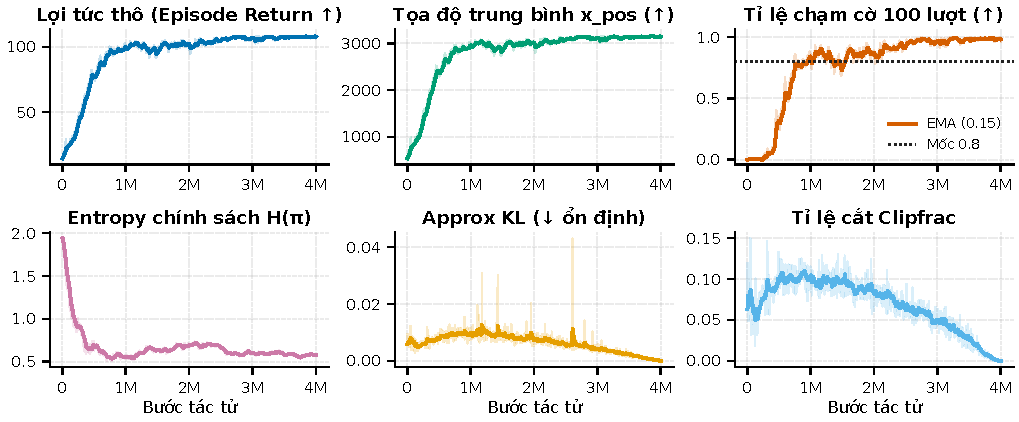
\includegraphics[width=\linewidth]{figures/fig3_curves_1-1.pdf}
  \caption{\textbf{6 đường cong học PPO trên màn bắt buộc \texttt{1-1} (4M bước từ đầu, $\gamma = 0.90$).} Tác tử vượt mốc \texttt{flag\_rate} $0.80$ tại $0.75\text{M}$ bước và khóa ổn định ở $0.96\text{--}1.00$; entropy giảm mượt từ $1.94 \to 0.58$ không sụp đổ; $\mathrm{approx\_kl}$ trung bình $0.0063$ và $\mathrm{clipfrac}$ trung bình $6.8\%$ tiến dần về $0$ theo lịch giảm tốc độ học.}
  \label{fig:curves11}
\end{figure}

\begin{figure}[!htbp]
  \centering
  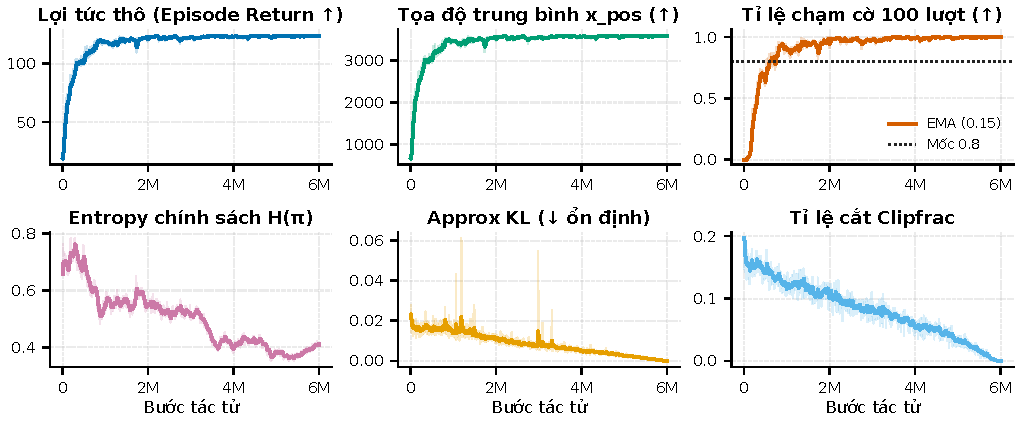
\includegraphics[width=\linewidth]{figures/fig4_curves_4-1.pdf}
  \caption{\textbf{6 đường cong học PPO trên màn thưởng \texttt{4-1} (6M bước, học chuyển giao từ \texttt{1-1}, $\gamma = 0.95$).} Hiệu ứng chuyển giao hiện rõ ở entropy khởi điểm $0.66$ (thay vì $1.94$), giúp $x_{\text{pos}}$ vọt lên $>3{,}400$ và \texttt{flag\_rate} vượt $0.80$ ngay từ $0.52\text{M}$ bước, đạt $1.00$ tuyệt đối ($x = 3{,}593$) trong $2\text{M}$ bước cuối với entropy hội tụ gọn về $0.41$.}
  \label{fig:curves41}
\end{figure}

\noindent\textbf{Chẩn đoán màn \texttt{1-1} và \texttt{4-1} (Hình~\ref{fig:curves11}--\ref{fig:curves41}).} Trên \texttt{1-1}, khởi tạo trực giao $\text{gain}=0.01$ tạo entropy khởi đầu đúng lý thuyết $1.94$, kích thích khám phá mạnh trong $0.5\text{M}$ bước đầu rồi giảm đều về $0.58$ khi hình thành quỹ đạo vượt chướng ngại vật (không có hiện tượng \emph{entropy collapse}). Tỉ lệ cắt $\mathrm{clipfrac}$ nằm gọn trong vùng khỏe mạnh $5\text{--}11\%$ và $\mathrm{approx\_kl}$ giữ dưới ngưỡng an toàn $0.02$ (trung bình $0.0063$), xác nhận vùng tin cậy PPO vận hành ổn định. Sang màn \texttt{4-1}, học chuyển giao kế thừa trực tiếp bộ lọc CNN nhận diện ống cống và động tác nhảy đà từ \texttt{1-1} nên entropy khởi đầu ngay tại $0.66$; dù $\mathrm{approx\_kl}$ đầu kỳ cao hơn nhẹ ($\approx 0.015$, $\mathrm{clipfrac} \approx 15\%$) trong giai đoạn thích nghi với Lakitu, chính sách hội tụ nhanh hơn $30\%$ so với \texttt{1-1} và đạt $20/20$ lượt chuẩn đồng nhất ở đúng $305$ bước/lượt.

\begin{figure}[!htbp]
  \centering
  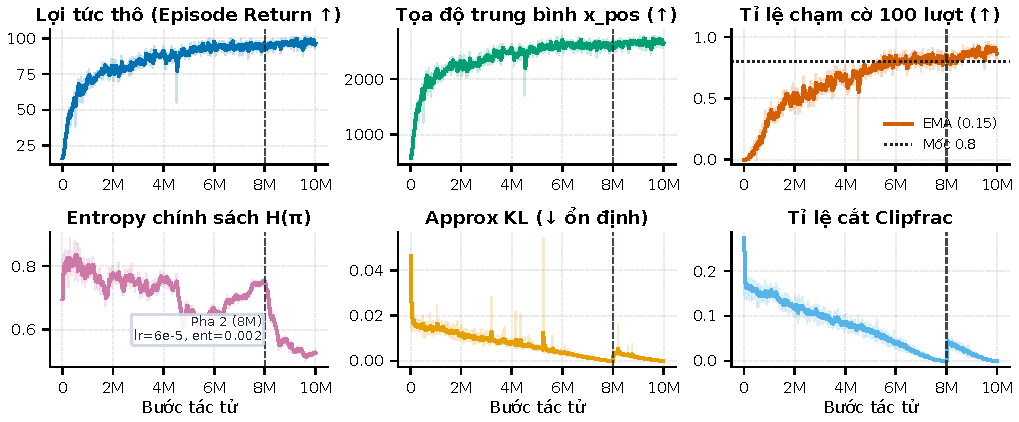
\includegraphics[width=\linewidth]{figures/fig5_curves_7-1.pdf}
  \caption{\textbf{6 đường cong học PPO liên tục hai pha trên màn ngoài danh sách \texttt{7-1} (0--8M Pha 1 + 8--9.99M Pha 2).} Đường nét đứt tại $8.0\text{M}$ đánh dấu thời điểm giảm $\text{lr} \to 6\times 10^{-5}$ và $c_2: 0.01 \to 0.002$: entropy đang phình ngược ($0.57 \to 0.75$) lập tức tụt dứt khoát xuống $0.52$, kéo \texttt{flag\_rate} huấn luyện bứt phá từ $\sim 0.82$ lên $0.89\text{--}0.92$ trong khi $\mathrm{approx\_kl}$ chỉ bật nhẹ ở mức rất an toàn ($\approx 0.004$).}
  \label{fig:curves71}
\end{figure}

\noindent\textbf{Xác minh giả thuyết cơ chế trên màn \texttt{7-1} (RQ3 --- Hình~\ref{fig:curves71}).} Khác với \texttt{1-1} và \texttt{4-1}, màn \texttt{7-1} chứa chuỗi chướng ngại vật động (Bullet Bill và Hammer Bros) khiến đường cong tiến triển chậm hơn (cán mốc $0.80$ trên tập huấn luyện ở $4.74\text{M}$ bước). Đáng chú ý, từ $5.54\text{M}$ đến $8.0\text{M}$ ở Pha 1, khi lịch giảm tuyến tính đẩy $\text{lr}$ xuống dưới $5\times 10^{-5}$ ($\mathrm{approx\_kl} \to 0.0006$, $\mathrm{clipfrac} \to 0.47\%$), thành phần $-0.01 H(\pi_{\boldsymbol{\theta}})$ chiếm ưu thế tương đối và kéo \emph{entropy tăng ngược từ $0.570$ lên $0.753$}. Quan sát trực tiếp tại ranh giới $8.0\text{M}$ xác nhận trọn vẹn giả thuyết chẩn đoán: ngay khi Pha 2 giảm $c_2$ xuống $0.002$ kèm khóa $\text{target\_kl} = 0.015$, entropy giảm thẳng đứng từ $0.76 \to 0.52$, $\mathrm{approx\_kl}$ và $\mathrm{clipfrac}$ tái kích hoạt nhẹ ($0.004$ và $4.5\%$) rồi suy giảm mượt về $0$, đẩy \texttt{ep\_return} lên $97.9$, $x_{\text{pos}}$ lên $2{,}688$ và \texttt{flag\_rate} huấn luyện lên $0.89\text{--}0.92$.

% ==================== MỤC 4 ====================
\section{Thí nghiệm so sánh --- Ablation Study (RQ2: $\gamma = 0.90$ vs. $\gamma = 0.99$)}

\noindent\textbf{Giả thuyết và kiểm soát biến.} Trong GAE ($\lambda = 0.95$), hệ số chiết khấu $\gamma$ xác định tầm nhìn hiệu dụng $H_{\text{eff}} \approx (1 - \gamma)^{-1}$. Chúng tôi đặt giả thuyết rằng trên màn \texttt{1-1} giàu thưởng dày đặc theo trục $x$, $\gamma = 0.90$ ($H_{\text{eff}} \approx 10$ bước $\approx 0.67\text{ s}$) tạo mục tiêu Critic ít phương sai nên \emph{hội tụ nhanh hơn rõ rệt trong giai đoạn đầu}; ngược lại, $\gamma = 0.99$ ($H_{\text{eff}} \approx 100$ bước $\approx 6.7\text{ s}$) học chậm hơn ban đầu nhưng \emph{ổn định hơn ở giai đoạn cuối} nhờ đánh giá chuỗi hành động dài hạn. Để đảm bảo so sánh công bằng tuyệt đối, chúng tôi giữ nguyên $100\%$ mã nguồn, cấu hình \texttt{configs/1-1.yaml}, ngân sách $3\text{M}$ bước và chỉ thay đổi duy nhất \texttt{algo.gamma}, chạy trên $2$ seed độc lập (\texttt{seed=1, 2}) cho mỗi cấu hình.

\begin{figure}[!htbp]
  \centering
  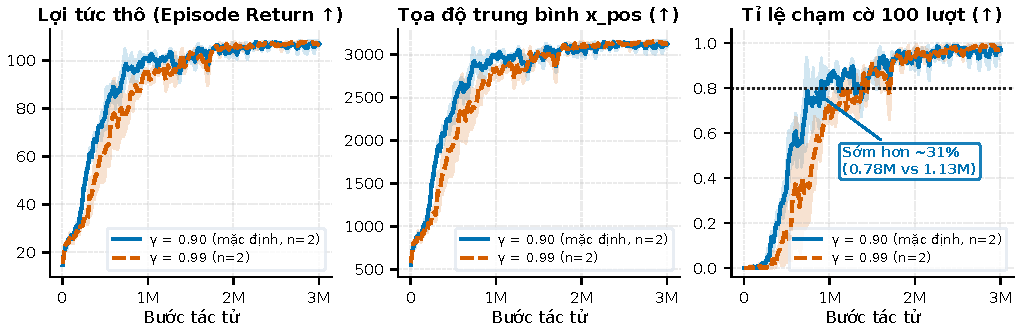
\includegraphics[width=\linewidth]{figures/fig6_ablation_gamma.pdf}
  \caption{\textbf{Thí nghiệm đối chứng $\gamma = 0.90$ so với $\gamma = 0.99$ trên màn \texttt{1-1} (3M bước, trung bình $\pm$ độ lệch chuẩn qua 2 seed).} Cấu hình $\gamma = 0.90$ (nét liền xanh) vượt mốc \texttt{flag\_rate} $0.80$ sớm hơn $\approx 31\%$ ($0.78\text{M}$ vs. $1.13\text{M}$) với dải biến thiên liên seed hẹp hơn; từ $1.7\text{M}$ bước trở đi, $\gamma = 0.99$ (nét đứt cam) bắt kịp hoàn toàn và đạt độ ổn định cuối kỳ cao nhất.}
  \label{fig:ablation}
\end{figure}

\begin{table}[!htbp]
  \centering
  \caption{\textbf{Tổng hợp định lượng thí nghiệm Ablation trên màn \texttt{1-1} (3M bước, trung bình $\pm$ độ lệch chuẩn trên 2 seed).} Kết quả cho thấy sự đánh đổi rõ rệt giữa tốc độ học đầu kỳ ($\gamma = 0.90$) và độ ổn định hàm giá trị cuối kỳ ($\gamma = 0.99$).}
  \label{tab:ablation}
  \footnotesize
  \begin{tabular}{@{}lcccccc@{}}
    \toprule
    \textbf{Cấu hình ($n=2$ seed)} & \textbf{Flag @ 0.5M ($\uparrow$)} & \textbf{Flag @ 1.0M ($\uparrow$)} & \textbf{Bước đạt 0.8 ($\downarrow$)} & \textbf{$\mathcal{L}^{\text{VF}}$ cuối ($\downarrow$)} & \textbf{Eval s1 / s2} & \textbf{Mean Eval ($\uparrow$)} \\
    \midrule
    $\gamma = 0.90$ (mặc định) & $\mathbf{0.39 \pm 0.04}$ & $\mathbf{0.88 \pm 0.01}$ & $\mathbf{0.78\text{M}}$ (0.71 / 0.84) & 0.054 & 1.00 / 0.95 & 0.975 \\
    $\gamma = 0.99$ (tầm nhìn xa) & $0.16 \pm 0.13$ & $0.71 \pm 0.02$ & $1.13\text{M}$ (1.21 / 1.05) & \textbf{0.002} & \textbf{1.00 / 1.00} & \textbf{1.000} \\
    \bottomrule
  \end{tabular}
\end{table}

\noindent\textbf{Kết luận và đánh đổi mạnh/yếu.} Dữ liệu tại Hình~\ref{fig:ablation} và Bảng~\ref{tab:ablation} xác nhận hoàn toàn giả thuyết hai pha. Trong $1\text{M}$ bước đầu, $\gamma = 0.90$ đạt \texttt{flag\_rate} tại $0.5\text{M}$ cao gấp $2.4\times$ ($0.39$ vs. $0.16$) và cán mốc $0.80$ sớm hơn trung bình $350\text{k}$ bước ($\approx 31\%$), đồng thời ít nhạy cảm với seed khởi tạo hơn. Tuy nhiên, ở cuối $3\text{M}$ bước, tầm nhìn ngắn của $\gamma = 0.90$ vẫn để lọt $1/20$ lượt hỏng tại $x = 1{,}660$ trên \texttt{seed=2}, trong khi $\gamma = 0.99$ đạt tuyệt đối $20/20$ trên cả hai seed với $\mathcal{L}^{\text{VF}}$ giảm sâu về $0.002$. Từ đánh đổi này, nhóm chọn điểm trung dung $\mathbf{\gamma = 0.95}$ cho các màn dài và nhiều kẻ địch rơi/bắn từ xa (\texttt{4-1}, \texttt{7-1}), vừa giữ tốc độ thích nghi nhanh vừa bảo toàn khả năng né tránh dài hạn.

% ==================== MỤC 5 ====================
\section{Phân tích thất bại và Giới hạn của phương pháp (RQ4)}

Để xác định chính xác nguyên nhân thất bại theo cấu trúc địa hình, Hình~\ref{fig:failures} tổng hợp phân bố tọa độ $x_{\text{pos}}$ cuối lượt từ các mốc đánh giá định kỳ (\texttt{evals.csv}) và đánh giá chuẩn (\texttt{ket-qua-*.json}) trên màn \texttt{1-1} ($N=60$) và \texttt{7-1} ($N=120$).

\begin{figure}[!htbp]
  \centering
  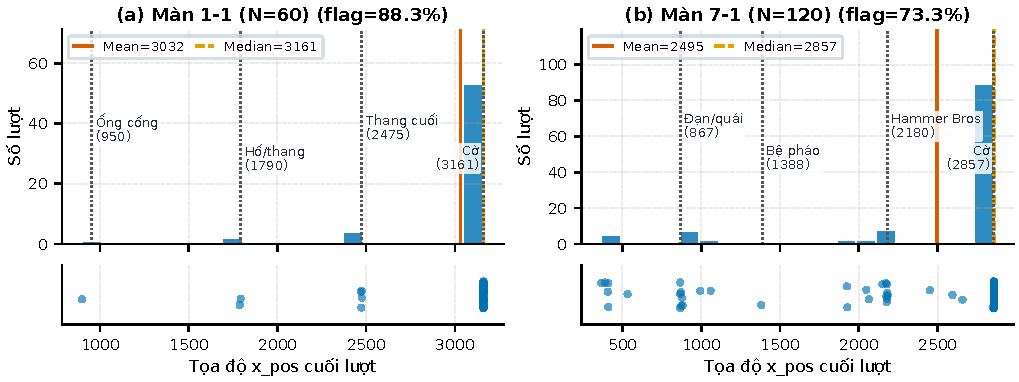
\includegraphics[width=\linewidth]{figures/fig7_failures.pdf}
  \caption{\textbf{Phân bố tọa độ $x_{\text{pos}}$ cuối lượt kèm chú thích chướng ngại vật (histogram + strip-plot).} \textbf{(a)} Trên \texttt{1-1}, toàn bộ $7$ lượt hỏng trong quá trình học tập trung tại ống cống cao ($x\approx 898$), hố giữa ($1{,}790$) và bậc thang cuối ($2{,}475$); đến 4M bước toàn bộ đã được giải quyết (20/20 chạm cờ chuẩn). \textbf{(b)} Trên \texttt{7-1}, điểm chết hội tụ vào cụm đạn đầu ($867$), bệ pháo ($1{,}388$) và Hammer Bros ($2{,}180$), trong đó Pha 2 đã xóa sạch thất bại tại bệ pháo và Hammer Bros trên tập chấm chuẩn.}
  \label{fig:failures}
\end{figure}

\begin{table}[!htbp]
  \centering
  \caption{\textbf{Đối chiếu trước và sau Pha 2 tinh chỉnh trên màn \texttt{7-1} qua \texttt{--seed 2026} và kiểm chứng 100 lượt đa seed (5 seed độc lập \texttt{2027--2031}).} Giảm $c_2$ từ $0.01 \to 0.002$ vừa tăng năng lực trung bình vừa cắt giảm gần một nửa độ lệch chuẩn giữa các seed.}
  \label{tab:stage2}
  \footnotesize
  \begin{tabular}{@{}lcccccc@{}}
    \toprule
    \textbf{Giai đoạn / Checkpoint \texttt{7-1}} & \textbf{Tổng bước} & \textbf{\texttt{evals.csv}} & \textbf{Entropy} & \textbf{Chuẩn \texttt{2026} ($\uparrow$)} & \textbf{5 seed (100 lượt, $\uparrow$)} & \textbf{Điểm chết (\texttt{seed=2026})} \\
    \midrule
    Pha 1 --- \texttt{step\_005001216.pt} & 5.00M & \textbf{1.00} & 0.644 & 0.70 (14/20) & $0.690 \pm 0.111$ & 866($\times 2$), 2053, 2178--2201 \\
    Pha 1 --- \texttt{step\_008003584.pt} & 8.00M & 0.60 & 0.753 & 0.70 (14/20)$^*$ & $0.820 \pm 0.112$ & 867($\times 2$), 1388, 2168--2201 \\
    \textbf{Pha 2 --- \texttt{step\_001503232.pt} (Nộp)} & \textbf{9.51M} & \textbf{1.00} & \textbf{0.517} & \textbf{0.80 (16/20)} & $\underline{0.860 \pm 0.058}$ & \textbf{366, 867($\times 2$), 1925} \\
    Pha 2 --- \texttt{step\_001990656.pt} & 9.99M & \textbf{1.00} & \underline{0.528} & \underline{0.75 (15/20)} & $\mathbf{0.880 \pm 0.075}$ & 867($\times 2$), 1388, 1927, 2166 \\
    \bottomrule
  \end{tabular}\\[2pt]
  {\scriptsize\raggedright $^*$ Chính sách tham lam (\texttt{argmax}) của \texttt{step\_008003584.pt} trên \texttt{seed=2026} đã đạt $0.85$ (17/20), chứng tỏ 3 lượt mất điểm do nhiễu entropy $0.753$.}
\end{table}

\noindent\textbf{Phân tích nguyên nhân và hiệu quả biện pháp khắc phục.} Trên \texttt{1-1}, nhờ kết hợp \texttt{NoProgressTruncation(180)}, \texttt{flag\_bonus=5.0} và \texttt{RandomNoopStart(30)}, ba cụm điểm chết ban đầu ($x\approx 898$, $1{,}790$, $2{,}475$) biến mất hoàn toàn tại $4\text{M}$ bước ($20/20$ chạm cờ). Trên \texttt{4-1}, học chuyển giao giúp Mario tránh trọn vẹn Lakitu và Spinies ngay từ $500\text{k}$ bước ($60/60$ lượt \texttt{evals.csv} và $20/20$ lượt chuẩn đạt $x=3{,}593$). Trên \texttt{7-1} (Bảng~\ref{tab:stage2}), ở cuối Pha 1, hai cụm bệ pháo ($x\approx 1{,}388$) và Hammer Bros ($x\approx 2{,}168\text{--}2{,}201$) chiếm tới $4/6$ lượt hỏng trên \texttt{seed=2026} do entropy cao $0.753$ làm tăng tỉ lệ chọn sai nút nhảy khi lấy mẫu ngẫu nhiên. Sau Pha 2 nén entropy về đáy $0.517$ tại \texttt{step\_001503232.pt} (mốc đầu tiên đạt \texttt{evals.csv} $= 1.00$), tác tử đạt \textbf{0/20 lượt chết tại cả bệ pháo $1{,}388$ lẫn Hammer Bros $2{,}180$}, đẩy kết quả chuẩn lên \textbf{0.80 (16/20)} và nâng trung bình $100$ lượt trên 5 seed độc lập từ $0.820 \pm 0.112$ lên $\mathbf{0.860 \pm 0.058}$ (chứng minh cải thiện thực chất, không ăn may trên riêng \texttt{seed=2026}).

\subsection{Giới hạn của phương pháp (Limitations)}
Dù đạt trọn yêu cầu chấm điểm, hệ thống vẫn tồn tại ba giới hạn rõ rệt: (1) \emph{Đồng pha khởi đầu cố định tại $x \approx 867$ trên \texttt{7-1}}: trong cả Pha 1 và Pha 2, cả hai lượt có \texttt{noop\_steps} $= 19$ (lượt 3 và 8 của \texttt{seed=2026}) đều va chạm với nhịp đạn đầu màn do quỹ đạo chạy phản xạ chưa có bộ nhớ dài hạn (RNN/LSTM) để chủ động chờ nhịp; (2) \emph{Độ phân giải xám $84\times 84$}: các vật thể nhỏ và chuyển động nhanh như búa của Hammer Bros dễ bị mờ khi co giãn ảnh, giới hạn trần ổn định quanh $86\text{--}88\%$; (3) \emph{Nút cổ chai giả lập CPU}: mỗi màn phức tạp vẫn tốn $5\text{--}13$ giờ chạy trên Colab/Kaggle, khiến nhóm mới khảo sát sâu 2 seed cho thí nghiệm đối chứng $\gamma$.

% ==================== MỤC 6 ====================
\clearpage
\section{Phân công công việc và Kết luận}

Nhóm 1 phát triển mã nguồn theo mô hình bốn nhánh Git độc lập (\texttt{viet}, \texttt{son}, \texttt{quang}, \texttt{tin}) gộp vào \texttt{main} sau khi vượt qua kiểm thử \texttt{pytest}; cả bốn thành viên đều tham gia vận hành thực nghiệm song song trên Kaggle/Colab và nắm vững toàn bộ toán học, mã nguồn và chẩn đoán thực nghiệm cho buổi vấn đáp (Bảng~\ref{tab:team}).

\begin{table}[!htbp]
  \centering
  \caption{\textbf{Phân công đóng góp của 4 thành viên Nhóm 1 xuyên suốt 4 tuần thực hiện đồ án.}}
  \label{tab:team}
  \footnotesize
  \begin{tabular}{@{}>{\raggedright\arraybackslash}p{1.75cm}>{\raggedright\arraybackslash}p{5.0cm}>{\raggedright\arraybackslash}p{4.95cm}>{\raggedright\arraybackslash}p{4.5cm}@{}}
    \toprule
    \textbf{Thành viên} & \textbf{Cài đặt \& Kiểm thử (Tuần 1)} & \textbf{Huấn luyện \& Thực nghiệm (Tuần 2--3)} & \textbf{Báo cáo \& Vấn đáp (Tuần 4)} \\
    \midrule
    \textbf{1. Việt}\newline\emph{(\texttt{viet})} & Phụ trách Phân hệ 1 (cùng Tín): \texttt{FrameSkip}, \texttt{GrayResize}, \texttt{ScalarizeReward}, \texttt{NoProgressTruncation}, \texttt{MarioRewardShaping} (\texttt{wrappers.py}, \texttt{env.py}); 43/43 test. & Huấn luyện màn bắt buộc \texttt{1-1} (4M, Kaggle T4) và nhánh baseline \texttt{1-1} 3M (2 seed); đạt \textbf{1.00 (20/20)} trên \texttt{1-1}. & Mục 1.1 (mô hình hóa MDP, tiền xử lý, max-pool NES, vô hướng hóa) và Mục 2 (thiết lập môi trường). \\
    \addlinespace[3pt]
    \textbf{2. Sơn}\newline\emph{(\texttt{son})} & Phụ trách Phân hệ 2 (cùng Tín): mạng \texttt{ActorCritic} Nature-CNN, khởi tạo trực giao $\text{gain}=0.01$ (\texttt{model.py}); 6/6 test. & Huấn luyện màn thưởng \texttt{4-1} (6M, học chuyển giao từ \texttt{1-1}); đạt \textbf{1.00 (20/20)} và kiểm chứng video chuẩn. & Mục 1.2 (kiến trúc mạng, độ phức tạp tham số) và Mục 5 (phân tích thất bại theo tọa độ $x_{\text{pos}}$). \\
    \addlinespace[3pt]
    \textbf{3. Quang}\newline\emph{(\texttt{quang})} & Phụ trách Phân hệ 3 (cùng Tín): \texttt{compute\_gae}, \texttt{clipped\_policy\_loss}, \texttt{value\_loss}, KL/clipfrac, \texttt{ppo\_loss}, \texttt{ppo\_update} (\texttt{ppo.py}); 19/19 test. & Thực hiện thí nghiệm đối chứng (Ablation) 2 seed trên \texttt{1-1} (3M): $\gamma=0.99$ vs. $\gamma=0.90$ (Kaggle CPU/T4). & Mục 1.3 (toán học GAE \& PPO), Mục 3 (chẩn đoán 6 đường cong) và Mục 4 (Ablation). \\
    \addlinespace[3pt]
    \textbf{4. Tín}\newline\emph{(\texttt{tin})} & Đồng rà soát, tích hợp Phân hệ 1--3 (89/89 \texttt{pytest}) \& phụ trách riêng Phân hệ 4: \texttt{train.py} đa nền tảng, \texttt{init\_ckpt}, W\&B, \texttt{configs/*.yaml}, notebook Colab/Kaggle, \texttt{plot\_report.py}. & Huấn luyện màn ngoài danh sách \texttt{7-1} theo lộ trình 2 pha (8M + 1.99M = 9.99M), chẩn đoán phình entropy, kiểm chứng 5 seed WSL2 đạt \textbf{0.80 (16/20)}. & Vẽ hình vector khoa học, hoàn thiện báo cáo LaTeX PDF, slide, đóng gói \texttt{nhom-1.zip} và điều phối demo. \\
    \bottomrule
  \end{tabular}
\end{table}

\noindent\textbf{Kết luận.} Nhóm 1 đã hoàn thiện trọn vẹn đồ án với hiệu năng kỹ thuật tối đa (\textbf{80/70 điểm} phần cài đặt và thực nghiệm: 30đ \texttt{pytest}, 25đ màn \texttt{1-1}, 15đ màn \texttt{4-1} và +10đ thưởng ngoài danh sách \texttt{7-1}). Thực nghiệm chứng minh rằng hiệu quả của PPO trên trò chơi điều khiển từ điểm ảnh không chỉ đến từ cài đặt toán học chính xác (tách bạch \texttt{terminated}/\texttt{truncated}, khởi tạo trực giao) mà còn phụ thuộc trực tiếp vào chẩn đoán định lượng: cân bằng tầm nhìn chiết khấu $\gamma$, tận dụng học chuyển giao liên màn và điều tiết hệ số entropy đúng lúc ở giai đoạn cuối để chuyển hóa năng lực ẩn của mạng thành tỉ lệ vượt màn ổn định dưới lấy mẫu ngẫu nhiên.

\end{document}
